\clearpage
\section{Градиентный граф}
Для организации процесса обучения нейронной сети было решено автоматически генерировать граф, позволяющий подсчитывать градиент на исходном графе. Это позволит пользователю не думать о процессе оптимизации заданной им функции, т.к. она будет решена библиотекой за него. Кроме того, такой подход упрощает преобразование графа в программный код, т.к. одна и та же логика компиляции графа может быть применена и к исходному графу, и к графу-градиенту. Тогда итерация обучения нейронной сети будет выглядеть так:
\begin{enumerate}
    \item Загрузка данных в входные вершины графа
    \item Вычисление графа
    \item Вычисление градиента
    \item Воздействие результатов вычисления градиента на параметры исходного графа
\end{enumerate}
\par
Покажем на примере что из себя представляет граф-градиент для ранее описанного графа сложения.
\begin{figure}[H]
    \centering
    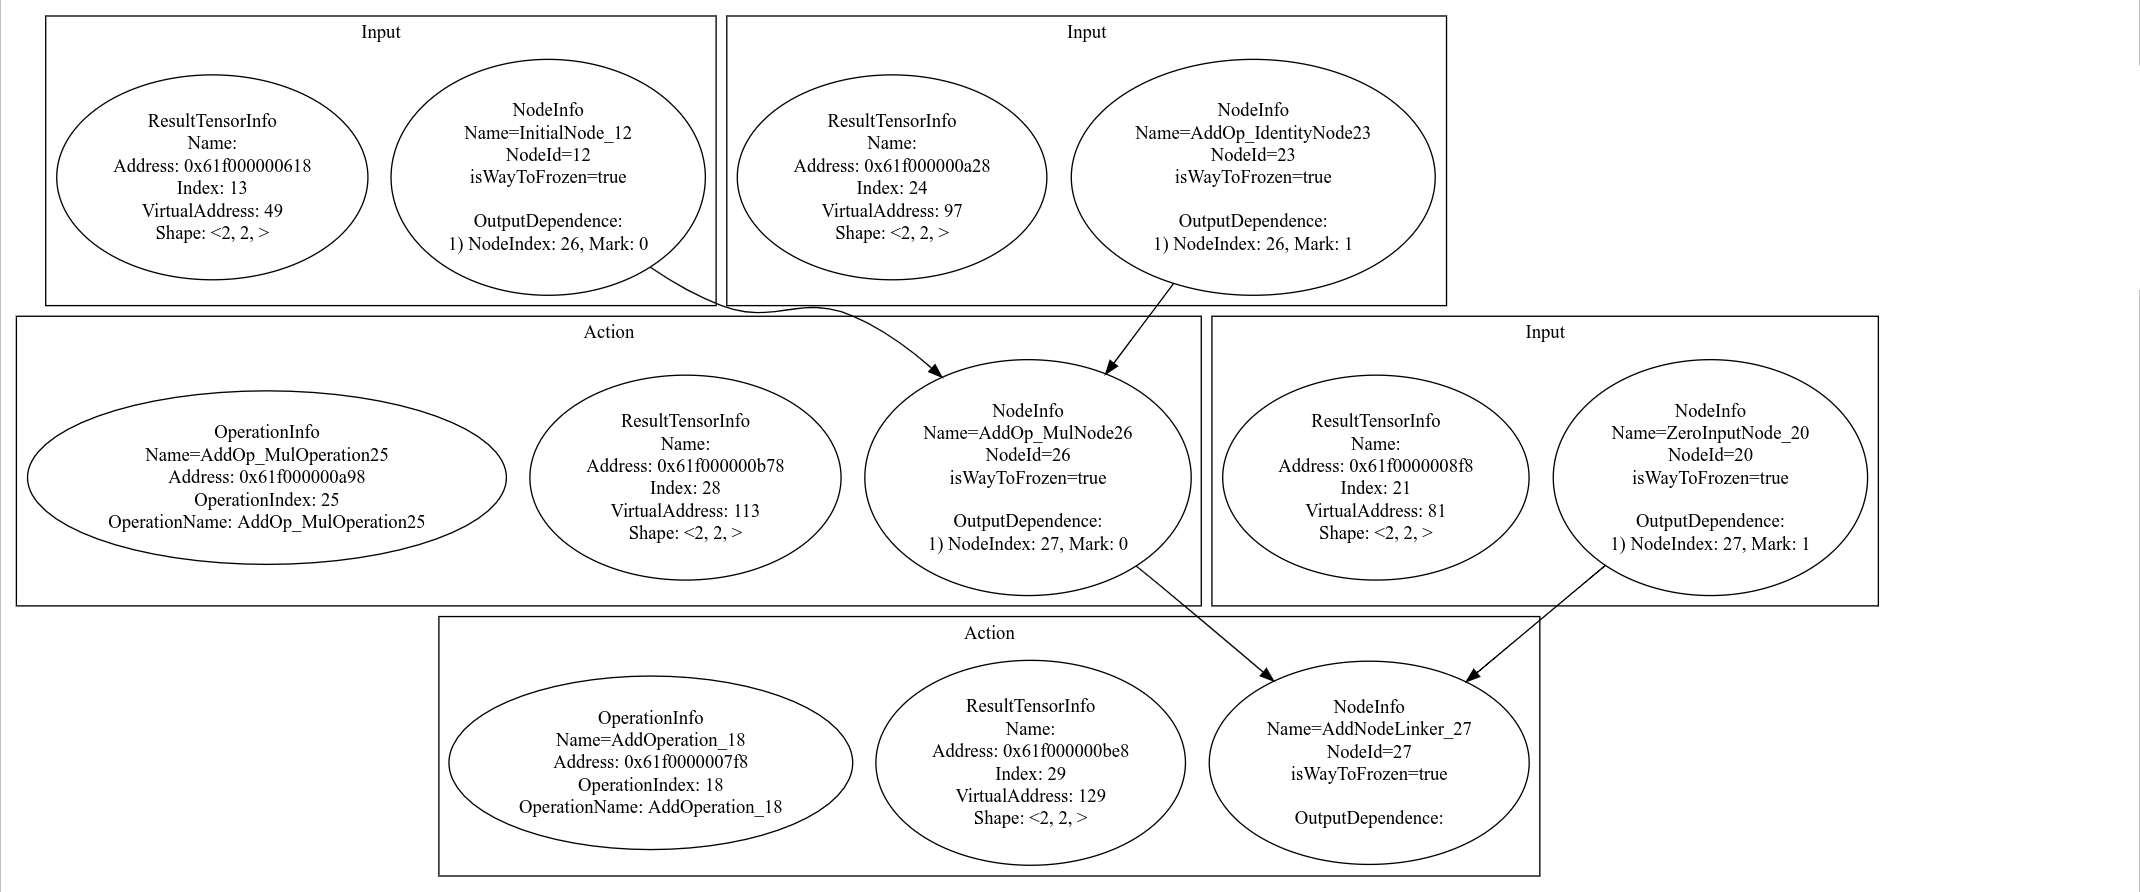
\includegraphics[width=0.8\textwidth]{GradientDotModel}
    \caption{Градиент графа сложения.}
    \label{GradientDotModel}
\end{figure}
